\begin{frame}{Monte Carlo Tree Search(MCTS)}{Quesque le MCTS}
	\begin{block}{}
		\begin{itemize}
			\item Le MCTS est un algorithme de recherche arborescente utilisé pour résoudre des problèmes afin de prendre une décision (un déplacement dans un jeu par exemple).
			\item Il n'utilise pas de fonction d'évaluation heuristique comparé à $\alpha$$\beta$ par exemple.
			\item Il utilise les méthodes de Monte Carlo pour améliorer son efficacité.
			\item Il possède des variantes, dépendant de leur utilisation, comme Coulom ou Kocsis and Szepesvari par exemple.
			\item Applicable si toutes les règles de l'application sont connus et si la longueur d'une partie et les gains ont une limite.	
		\end{itemize}
	\end{block}
\end{frame}

\begin{frame}{Monte Carlo Tree Search(MCTS)}{Structure}
	\begin{block}{Arbre de recherche}
		\begin{itemize}
			\item L'arbre de recherche est une modélisation des possibilités de jeu pour la simulation.
			\item Un noeud représente un état du jeu.
			\item Chaque noeuds possèdent deux informations :
			\item\begin{itemize}
				\item - La valeur de sa position (dans un jeu, représenté souvent par la moyenne des résultats pour un jeu sur les noeuds visités)
				\item - Le nombre de visite de ce noeud dans la simulation
			\end{itemize}
			\item Chaque feuille de cet arbre représente soit un noeud dont les enfants n'ont pas encore été explorés, soit un état final de celui-ci.		
		\end{itemize}
	\end{block}
\end{frame}

\begin{frame}{Monte Carlo Tree Search(MCTS)}{Structure}
    \begin{block}{Plusieurs étapes}
	    	\begin{itemize}
	    		\item 1. Sélection
	    		\item 2. Expansion
	    		\item 3. Simulation
	    		\item 4. Rétropropagation
	    		\item Répété jusqu'à un certain temps jusqu'à la prise de décision.
	    	\end{itemize}
		\begin{center}
			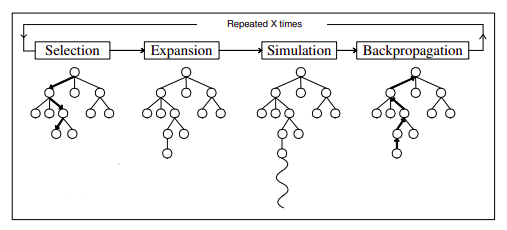
\includegraphics[width=8cm]{ressources/MCTSEtapes}
		\end{center}
	\end{block}
\end{frame}

\begin{frame}{Sélection}
\end{frame}

\begin{frame}{Expansion}
\end{frame}

\begin{frame}{Simulation}
\end{frame}

\begin{frame}{Rétropropagation}
\end{frame}